\hsection{Iteration, Comprehension, and Generators}%
\label{sec:iteration}%
%
In \python, iterating over the items in a sequence is a central concept.
In \cref{sec:enumOverSequences}, we learned that we can iterate over collections such as lists, tuples, dictionaries, and sets.
We can also iterate over the characters in a string in the same way.
These are all datastructures whose complete content exists in memory at any given time.
In \python, we can also iterate over sequences where the items that are constructed at the time when they are actually needed.
A good example for this is the \pythonilIdx{range} datatype.
We can iterate over all the 1\decSep000\decSep000\decSep000\decSep000 \pythonil{int} elements of \pythonil{range(100_000_000_000_000)} in a loop.
These many integers do not all exist in memory at the same time.
Instead, they are allocated and provided one-by-one as needed.
From the perspective of a programmer, we can iterate over \pythonilsIdx{range} and \pythonilsIdx{list} in exactly the same way.
Matter of fact, many objects in \python\ support iteration.

Vice versa, we can also create instances of collection datatypes from sequences of items.
For example, the datatypes \pythonilIdx{list}, \pythonilIdx{tuple}, \pythonilIdx{set}, and \pythonilIdx{dict} can also be used like functions that take a sequence of items as parameter and create an instance of the corresponding datatype.
In \cref{sec:lists}, we learned that \pythonil{[1, 2, 2, 3]} is a list \pgls{literal} with the specified contents.
Passing this list to the \pythonilIdx{set} function/datatype, i.e., writing \pythonil{set([1, 2, 2, 3])} will create the set \pythonil{\{1, 2, 3\}}.
We also learned that collection datastructures often have methods that allow us to modify in place by passing in other collections as arguments.
Invoking \pythonil{l.extend(\{1, 2, 3\})}\pythonIdx{list!extend}\pythonIdx{extend} will append the elements~\pythonil{1}, \pythonil{2}, and \pythonil{3} to a list~\pythonil{l}, for example.

\begin{figure}%
\centering%
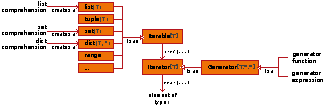
\includegraphics[width=0.96\linewidth]{\currentDir/iteration.pdf}%
\caption{The concepts of comprehension, \pythonilsIdx{Iterable}, \pythonilsIdx{Iterator}, and \pythonilsIdx{Generator} in \python.}%
\label{fig:iteration}%
\end{figure}%

You will very often encounter situations where you transform, process, or create sequences of data elements.
As sketched in \cref{fig:iteration}, there are many different manifestations of the concepts of \emph{iterating} over objects that are \emph{iterable} in \python.

The most primitive concept is the \pythonilIdx{Iterator}~\cite{PEP234,PSF:P3D:TPSL:BIT:IT,PSF:P3D:G:I2}.
This is an object that represents one visitation of a sequence of items.
If you have an \pythonilIdx{Iterator} object~\pythonil{u}, then you can get the next item from the sequence it represents by calling \pythonil{next(u)}.
If there is no next element, this will raise an \pythonil{StopIteration}.
Such iterators are single-use, one-pass objects.
A \pythonil{for} loop, for example, will consume elements from an \pythonilIdx{Iterator} until the \pythonil{StopIteration} is raised.
\pythonilIdx{Generator} expressions and functions are special \pythonilsIdx{Iterator} allowing us more control and a simpler syntax for defining element sequences, respectively.

Many datastructures like collections allow us to visit their elements as often as we wish.
They are instances of the \pythonilIdx{Iterable} interface.
We can invoke \pythonil{iter(coll)} on a collection \pythonil{coll} implementing this \pythonilIdx{Iterable}~\cite{PSF:P3D:G:I1} iterface and will get an \pythonilIdx{Iterator}.
Whenever we iterate over a list, a new \pythonilIdx{Iterator} is created this way.

As a side note, the operator \pythonilIdx{iter} can also be applied to an \pythonilIdx{Iterator}, not just to an \pythonilIdx{Iterable}~\cite{PSF:P3D:TPSL:BIT:IT}.
If applied to an \pythonilIdx{Iterator}, it returns the iterator itself~\cite{PSF:P3D:G:I2}.
Hence, all \pglspl{API} that require an \pythonilIdx{Iterable} as parameter and \emph{use it only once} can also accept an \pythonilIdx{Iterator}.

Finally, we can also create collections like lists, sets, and dictionaries via so-called \emph{comprehension}.
A~comprehension basically means writing a \pythonil{for} loop \emph{into} the corresponding collection literal.
It is a more compact and more efficient syntax to construct collections.
In this chapter, we will investigate all of these concepts beyond what we did not yet already discuss in \cref{sec:enumOverSequences,sec:collections}.%
%
\hsection{\texttt{Iterable}s and \texttt{Iterator}s}%
\label{sec:iterable}%
%
\gitEvalPython{iteration:list_iteration}{}{iteration/list_iteration.py}%
\listingBox{exec:iteration:list_iteration}{Manually iterating over a \pythonilIdx{list}.}{,style=python_console_style}%
%
\gitLoadAndExecPython{iteration:set_iteration}{}{iteration}{set_iteration.py}{}%
\gitExecPython{iteration:set_iteration_2}{}{iteration}{set_iteration.py}%
%
\listingPythonAndOutput{iteration:set_iteration}{%
Iterating over a set and the result: %
Every time we run the program, the output is likely to be different.%
Compare \cref{exec:iteration:set_iteration} and \cref{exec:iteration:set_iteration_2} and you will see that they are (probably) different.}{}%
\listingBox{exec:iteration:set_iteration_2}{Execuring program \programUrl{iteration:set_iteration} a second time. This time, the output should be different from \cref{exec:iteration:set_iteration}.}{,style=text_style}%
%
\gitEvalPython{iteration:range_iteration}{}{iteration/range_iteration.py}%
\listingBox{exec:iteration:range_iteration}{Manually iterating over a \pythonilIdx{range}, in exactly the same way that we used in \cref{exec:iteration:list_iteration}.}{,style=python_console_style}%
%
\begin{sloppypar}%
Any object that allows us to access its elements one-by-one, i.e., \emph{iteratively} is an instance of \pythonilIdx{typing.Iterable}\pythonIdx{Iterable}.
The actual iteration over the contents is then done by an \pythonilIdx{typing.Iterator}\pythonIdx{Iterator}~\cite{PEP234,PSF:P3D:TPSL:BIT:IT,PSF:P3D:G:I2}.
This distinction is necessary because we want to allow some objects to be iterated over multiple times.%
\end{sloppypar}%
%
Let's say you have the list \pythonil{x = ["a", "b", "c"]}, as in \cref{exec:iteration:list_iteration}.
We can use this list~\pythonil{x} in \pythonil{for xi in x}-kind of loops arbitrarily often.
We use \pythonil{x} in two different such \pythonil{for} loops.
\pythonil{x} is an instance of \pythonilIdx{list} and every list is also an instance
of~\pythonilIdx{Iterable}\pythonIdx{typing.Iterable}~\cite{PSF:P3D:G:I1}.
We show this by first importing the type \pythonilIdx{Iterable} from package \pythonilIdx{typing}.
As we already learned, the operator \pythonil{isinstance(obj, tpe)} returns \pythonil{True} if object \pythonil{obj} is an instance of type \pythonil{tpe}.
\pythonil{isinstance(x, Iterable)}\pythonIdx{isinstance} is therefore \pythonil{True}, because the list~\pythonil{x} can be iterated over.

Every time we do loop over \pythonil{x}, an \pythonilIdx{Iterator} instance is created internally by~(doing something like)~invoking~\pythonil{u = iter(x)}\pythonIdx{iter}.
To verify whether \pythonil{u} really is an instance of the ominous type \pythonilIdx{Iterator}, we first import this type from the package \pythonilIdx{typing}.
Then we invoke \pythonil{isinstance(u, Iterator)}\pythonIdx{isinstance}, which returns \pythonil{True}.
More precisely, the actual type of \pythonil{u} is \pythonil{list_iterator}\pythonIdx{list\_iterator}, which is a special implementation of \pythonilIdx{Iterator}.
You see, if we want to represent one step-by-step pass over the sequence~\pythonil{x}, then all we have to store in an object~\pythonil{u} is a reference to the list~\pythonil{x} we are iterating over as well as the current position, i.e., the index of the current element, in the iteration sequence.
\pythonil{list_iterator}\pythonIdx{list\_iterator}, does exactly that internally.

Every time a loop needs to advance to the next element~\pythonil{xi} in the sequence represented by \pythonil{u}, it does~(something like)~\pythonil{xi = next(u)}.
This will then yield the element at the current iteration index and advance the index by one.
The \pythonilIdx{for}~loop basically does this internally.

However, we can also do it \inQuotes{by hand.}
In \cref{exec:iteration:list_iteration}, we perform \pythonil{u = iter(x)} and \pythonil{v = iter(x)}.
This creates two independent \pythonilsIdx{Iterator}, i.e., two independent instances of \pythonil{list_iterator}\pythonIdx{list\_iterator},, which we can use to step over the list separately.
Each of them remembers a reference to list \pythonil{x} as well as its own iteration index.
Invoking \pythonil{next(u)}\pythonIdx{next} will yield the first element of the list~\pythonil{x}, namely~\pythonil{\"a\"}.
Calling \pythonil{next(u)}\pythonIdx{next} again gives us the second element, that is~\pythonil{\"b\"}.
If we now call \pythonil{next(v)}\pythonIdx{next}, i.e., apply~\pythonilIdx{next} to the second, independent \pythonilIdx{Iterator}, we again obtain the first element~(\pythonil{\"a\"}).

This again shows us why there is a distinction between the two \pglspl{API} \pythonilIdx{Iterable} and \pythonilIdx{Iterator}.
The former is interface that objects need to support it they holds or can generate a data sequence that can iteratively be visited.
The latter is provided by one independent iteration over such sequence.

The third invocation of \pythonil{next(u)}\pythonIdx{next} gives us~\pythonil{\"c\"}, the third and last element of~\pythonil{x}.
If we now call \pythonil{next(u)}\pythonIdx{next} a fourth time, something interesting happens:
A \pythonilIdx{StopIteration} is raised\pythonIdx{raise}.
Different from the exceptions that we already learned about, this is not an error at all.
This instead is how the end of an iteration sequence is signaled.
A \pythonilIdx{for}~loop will, for instance, stop when it encounters this exception.
If \pythonil{next(u)}\pythonIdx{next} is the way to get the next element from \pythonilIdx{Iterator}~\pythonil{u}, then there must also be some way to signal that the end of the sequence is reached.
Returning \pythonil{None} would not work, because a sequence may actually contain that value.
Therefore, the designers of \python\ simply chose to use the exception mechanism for this.

This approach to iterate over collections~\pythonil{col} by first creating an iterator~\pythonil{it} using the \pythonilIdx{iter} function as \pythonil{it = iter(col)} and then applying \pythonilIdx{next} to that iterator like \pythonil{next(it)} works for \pythonilsIdx{list} and \pythonilsIdx{tuple} alike.
It also works for \pythonilsIdx{set}, but be aware that the order in which the elements of a \pythonilIdx{set} are presented is not defined.
Back in \cref{bp:setsUnordered} we already clarified that \pythonilsIdx{set} are unordered data structures.
We explore this with program \programUrl{iteration:set_iteration} in \cref{lst:iteration:set_iteration}, which we execute twice, giving us the different outputs \cref{exec:iteration:set_iteration,exec:iteration:set_iteration_2}.
Interestingly, we can also iterate over \pythonilsIdx{dict}.
This iteration \emph{only} returns the dictionary keys however.
If we need the values or the key-value pairs of a dictionary~\pythonil{d}, then we have to iterate over \pythonil{d.values()}\pythonIdx{values}\pythonIdx{dict.values} or \pythonil{d.items()}\pythonIdx{items}\pythonIdx{dict.items}, respectively.

\Cref{exec:iteration:range_iteration} shows us that even \pythonilsIdx{range} have the exactly same behavior as \pythonilsIdx{list} with respect to iteration.
And they should, of course, like every other object that implements the~\pythonilIdx{Iterable} functionality.
Because of this, the \pythonil{for y in x}-type of loops can be applied to any \pythonilIdx{Iterable} or \pythonilIdx{Iterator} instance~\pythonil{x}.%
A \pythonilIdx{range} is basically a collection.
Different from the other collection types we know, its elements are not all explicitly created and stored.
Instead, they are created on the fly by the \pythonil{Iterator} objects that return them.
In our example, we construct a range~\pythonil{x} of the three number~0 to~2.
We then explore and iterate over it in exactly the same way we applied in \cref{exec:iteration:range_iteration}.
The only differences are that we now output numbers instead of strings and that the type of the iterator is \pythonil{range_iterator}\pythonIdx{range\_iterator}.

With this, we now know the how \pythonil{for} loops in \python\ actually work.
They create an iterator over a sequence and then consume the elements of this iterator, each time executing the loop body, until hitting a \pythonilIdx{StopIteration} exception.
All collection classes in \python\ that offer a sequential view on their data therefore support the \pythonilIdx{Iterable}/\pythonilIdx{Iterator}-\pgls{API}~\cite{PEP234}.
Due to this \pgls{API} structure, it is not even necessary to hold all the elements of a collection in memory at any point in time, as long as we can compute them as need.
An example for this is are \pythonilsIdx{range}, which provide us with \pythonil{int}-sequences with arbitrarily many numbers that are create~(and discarded) one-by-one during the iteration.%
%
\FloatBarrier%
\endhsection%
%
\hsection{List Comprehension}%
\label{sec:listComprehension}%
%
We can create a list by writing it down as a \pgls{literal}.
For example, \pythonil{[1, 2, 3, 4, 5]} creates a list\pythonIdx{list} containing the first five natural numbers.
This is very handy, but can also become cumbersome if we either have many elements or want to transform them.
Needing to write a \pgls{literal} in the same way that creates a list with the first one hundred natural numbers may be somewhat annoying.
If we want to create a list with the logarithms of first five natural numbers.
Writing something like \pythonil{[log(1), log(2), log(3), log(4), log(5)]}\pythonIdx{log} looks clunky as well.
Luckily, \python\ offers the much more convenient syntax of list comprehension\pythonIdx{list!comprehension}\pythonIdx{comprehension!list}~\cite{PEP202}:%
%
\pythonSyntax{syntax/list_comprehension.py}%
\FloatBarrier%
%
\gitLoadAndExecPython{iteration:simple_list_comprehension}{}{iteration}{simple_list_comprehension.py}{}%
\listingPythonAndOutput{iteration:simple_list_comprehension}{%
Some simple examples for list comprehension\pythonIdx{list!comprehension}\pythonIdx{comprehension!list}.}{}%
%
\gitExec{exec:iteration:simple_list_comprehension:ruff}{\programmingWithPythonCodeRepo}{.}{_scripts_/ruff.sh iteration simple_list_comprehension.py}%
\listingToolOutput{iteration:simple_list_comprehension:ruff}{%
The output of \ruff\ for the examples for list comprehension in \cref{lst:iteration:simple_list_comprehension}: %
The \pythonilIdx{for}~loop constructing the list \textil{squares_1} can indeed by replaced by a list comprehension\pythonIdx{list!comprehension}\pythonIdx{comprehension!list}.}%
%
This syntax creates a new list whose contents are the results of applying a given \pythonil{expression} to the items~\pythonil{item} of a \pythonil{sequence}.
You can imagine it as a \pythonil{for} loop where each iteration produces a value which is then stored in a list.
For example, \pythonil{[i for i in range(10)]} creates a list with the integer numbers~\pythonil{0} to~\pythonil{9}.
The list comprehension \pythonil{[i ** 2 for i in range(10)]} instead creates a list with the squares of these numbers (where \inQuotes{squaring} is the before-mentioned expression).

Optionally, we can select the elements that we want to have in the list by adding an \pythonilIdx{if}~clause.
\pythonil{[i for i in range(10) if i != 3]}, for instance, excludes the number~\pythonil{3} from our list.
Interestingly, the sequence over which the list creation iterates can itself also be such a comprehension expression.
It is totally fine to write \pythonil{[i * j for i in range(2) for j in range(2)]}, which yields \pythonil{[0, 0, 0, 1]} because both~\pythonil{i} and~\pythonil{j} will take on the values~\pythonil{0} and~\pythonil{1} independently of each other.

In \cref{lst:iteration:simple_list_comprehension} we provide some examples for list comprehension.
First, we want to construct a list with the squares of the integer numbers from~0 to~10.
Before learning about list comprehension, we would do this with a good old plain \pythonil{for} loop.
We would start by initially creating an empty list~\pythonil{squares_1}.
In a \pythonilIdx{for}~loop letting a variable~\pythonil{i} iterate over the \pythonil{range(0, 11)}\pythonIdx{range}.
In the body of the loop, we would then append \pythonil{i ** 2} to the list~\pythonil{squares_1} by invoking~\pythonil{squares_1.append(i ** 2)}\pythonIdx{list!append}\pythonIdx{append}.
This will occupy at least three lines of code.
But it works.
However, instead, we could write the comprehension expression \pythonil{[j ** 2 for j in range(11)]}, which achieves exactly the same thing only using a single line of code.

We can also select which elements of a sequence we want to insert into our list by using an \pythonilIdx{if} statement during the list comprehension.
In \cref{lst:iteration:simple_list_comprehension}, we demonstrate this by creating a list of even numbers from the range~0 to~9.
We let a variable~\pythonil{k} iterate over the \pythonil{range(10)}\pythonIdx{range}.
This lets~\pythonil{k} take on the values~\pythonil{0}, \pythonil{1}, \pythonil{2}, \dots, \pythonil{8}, and finally~\pythonil{9}.
Out of these values, we select only those for which \pythonil{k \% 2 == 0} via the \pythonilIdx{if}~statement.
In other words, we compute the result of the \pgls{modulodiv} of \pythonil{k} and~\pythonil{2}, i.e., the remainder of that division.
If it is zero, then \pythonil{k} is divisible by~\pythonil{2} and thus even.
Yes, yes, I know {\dots} of course, we could easily achieve the same result without the \pythonil{if} here by simply changing the range in the comprehension to \pythonil{range(0, 10, 2)} {\dots} or by just doing \pythonil{list(range(0, 10, 2))}.
It is just an example.
Anyway, we obtain the list~\pythonil{[0, 2, 4, 6, 8]}.

Finally, we play around with \inQuotes{nested} comprehension.
Let's say you have two \pythonilsIdx{Iterable} and want to produce all possible combinations of their output.
Side note:~Interestingly, \pythonilIdx{str} is also an \pythonilIdx{Iterable}.
You can iterate over the characters of a string.

Assume that the first sequence by~\pythonil{"abc"} and the second one be~\pythonil{"xy"}.
How can we create a list of all possible pairs that containing one letter from each of these strings?
By simply writing two \pythonil{for}~statements!
In \cref{lst:iteration:simple_list_comprehension}, we create the list~\pythonil{combinations} this way.
We write \pythonil{[f"\{m\}\{n\}" for m in "abc" for n in "xy"]}.
This lets the variable~\pythonil{m} take on, as value, each of the characters in the string~\pythonil{"abc"}, one by one.
For each of the values that~\pythonil{m} takes on, the variable~\pythonil{n} iterates over \pythonil{"xy"} and thus first becomes~\pythonil{"x"} and then~\pythonil{"y"}.
The \pgls{fstring} \pythonil{f"\{m\}\{n\}"} is \glslink{strinterpolation}{interpoliert} for each combination of~\pythonil{m} and~\pythonil{n}.
The result is thus the list~\pythonil{["ax", "ay", "bx", "by", "cx", "cy"]}.%
%
\begin{sloppypar}%
Of course, we can create lists of arbitrary datatypes using list comprehension.
These include also other lists, tuples, sets, dictionaries -- whatever we want.
We can repeat the above example and, instead of storing the combinations of characters as strings, we could store them as \pythonilsIdx{tuple}.
The list comprehension~\pythonil{[(o, p) for o in "abc" for p in "xy"]} does this.
It produces~\pythonil{[(\"a\", \"x\"), (\"a\", \"y\"), (\"b\", \"x\"), (\"b\", \"y\"), (\"c\", \"x\"), (\"c\", \"y\")]}.
\end{sloppypar}%
%
In \cref{exec:iteration:simple_list_comprehension:ruff}, we present the output that \ruff, our \cref{ut:ruff}, produces when we apply it to \programUrl{iteration:simple_list_comprehension} from \cref{lst:iteration:simple_list_comprehension}.
Interestingly, \ruff\ considers the construction of a list via the \pythonilIdx{append}\pythonIdx{list!append} function in a loop as a \emph{performance issue}, signified by the error prefix~\textil{PERF}.
This is, of course, only the case if the list could as well be constructed without calling \pythonilIdx{append} in a loop.
Well, we do know another way:
We can create the list via list comprehension, which is not always possible.
When it can be done, as is the case in our example, we noticed that list comprehension is more compact.
Code which is more compact is often more readable and in this case, from a software engineering point of view, often preferable.
But why would the original loop also be an issue of performance, i.e., execution speed?

\gitLoadAndExecPython{iteration:list_of_numbers_append}{}{iteration}{list_of_numbers_append.py}{}%
\listingPythonAndOutput{iteration:list_of_numbers_append}{%
Create a \pythonilIdx{list} with the even numbers from~0 to~1\decSep000\decSep000 using the \pythonilIdx{append}.}{}%
%
\gitLoadAndExecPython{iteration:list_of_numbers_comprehension}{}{iteration}{list_of_numbers_comprehension.py}{}%
\listingPythonAndOutput{iteration:list_of_numbers_comprehension}{%
Create a \pythonilIdx{list} with the even numbers from~0 to~1\decSep000\decSep000 using list comprehension.}{}%

OK, let's try to verify this.
In order to investigate this issue, we could try to simply create two lists with the same contents.
We would create one by using the \pythonilIdx{append} method in a loop and one by using list comprehension.
Very much like what we did just now.
Whichever is faster, i.e., needs less time, has the better performance.

Now measuring the runtime needed by something is always a dodgy subject.
The runtime of a \python\ program obviously depends on the machine and CPU it is running on.
It is also affected by the operating system, the available RAM, the disk speed, and of course by other processes running on the same machine at the same time~\cite{WCLTTCMY2014BOAAOSFFTTSP}.
Clearly, it also depends on which version of the \python\ interpreter we use and our results of the measurement could be different after each software update.
So every runtime measurement is always fuzzy and imprecise~\cite{WCLTTCMY2014BOAAOSFFTTSP}.
Whatever we would measure would have to take with a grain of salt, but we will try it anyway.%
%
\usefulTool{timeit}{%
\pythonilIdx{timeit} is a tool for measuring execution time of small code snippets that ships directly with \python. %
This module avoids a number of common traps for measuring execution times, see~\cite{PSF:P3D:TPSL:TMETOSCS,P2002AI}.%
}%
%
\pythonilIdx{timeit} allows us to measure the runtime of a certain statement.
We want to measure how long it takes to create a list containing all even numbers from~\intRange{0}{1\decSep000\decSep000}.

In \cref{lst:iteration:list_of_numbers_append} we therefore first implement a function \pythonil{create_by_append} which constructs the list using the \pythonilIdx{append}\pythonIdx{list!append} method in a loop.
In a loop over the \pythonil{range(1_000_001)}, it appends all the even numbers to the list \pythonil{numbers}.
Finally, it returns the list.

To measure the runtime of this function, we first \pythonilIdx{import} the function \pythonilIdx{repeat}\pythonIdx{timeit!repeat} from the module~\pythonilIdx{timeit}.
We tell \pythonilIdx{repeat} to call our function \pythonil{create_by_append} one time~(\pythonil{number=1}) and measure the consumed runtime.
It will return the runtime in seconds and stored as a \pythonil{float}.
However, factors like those mentioned above, scheduling by the operating system, maybe garbage collection by the \python\ iterpreter, and so on, a single measurement would not be very reliable~\cite{P2002AI}.
We thus instruct \pythonilIdx{repeat} function to take 90 such measurements~(argument \pythonil{repeat=90}).
All of the measured runtimes are then return as a \pythonil{list[float]}.
The documentation of \pythonilIdx{timeit}~\cite{PSF:P3D:TPSL:TMETOSCS} says:%
%
\cquotation{PSF:P3D:TPSL:TMETOSCS}{%
\emph{Note:}~it's tempting to calculate mean and standard deviation from the result vector and report these.
However, this is not very useful.
In a typical case, the lowest value gives a lower bound for how fast your machine can run the given code snippet;
higher values in the result vector are typically not caused by variability in \python's speed, but by other processes interfering with your timing accuracy.
So the \pythonil{min()}\pythonIdx{min} of the result is probably the only number you should be interested in.
After that, you should look at the entire vector and apply common sense rather than statistics.%
}%
%
\bestPractice{timeMeasurement}{%
When measuring the runtime of code for one specific set of inputs, it makes sense to perform multiple measurements and to take the \emph{minimum} of the observed values~\cite{PSF:P3D:TPSL:TMETOSCS}. %
The reason is that there are many factors~(CPU temperature, other processes, \dots) that may \emph{negatively} impact the runtime. %
However, there is no factor that can make your code faster than what your hardware permits. %
So the minimum is likely to give the most accurate impression of how fast your code can theoretically run on your machine. %
Notice, however, that there might be effects such as caching that could corrupt your measurements.%
}%
%
So we do just that.
\pythonilIdx{repeat} gives us a list with measured runtimes.
The \pythonilIdx{min} function accepts a sequence of elements and returns the smallest one~\cite{PSF:P3D:TPSL:BIF}.
Thus, we print the result of \pythonilIdx{min} applied to the list returned by \pythonilIdx{repeat}.
We format the output to be in milliseconds and rounded to three digits, to be a bit more readable.
The result can be seen in \cref{exec:iteration:list_of_numbers_append}.

Now the \pgls{formatPDF} document of this book is built automatically using a \github~Action~\cite{C2024GA}.
This action executes all the \python\ example programs and weaves their output into the book.
Everytime I update the book, this process is repeated.
This means that, when writing this text, I do not know what value you will see in \cref{exec:iteration:list_of_numbers_append}.
On my local machine, I get \textil{runtime/call: 30.1 ms.}

Anyway, in order to test whether list comprehension is really faster than iterative list construction via \pythonilIdx{append}\pythonIdx{list!append}, we now write the second program \cref{lst:iteration:list_of_numbers_comprehension}.
This program is very similar to \cref{lst:iteration:list_of_numbers_append}.
It defines a function \pythonil{create_by_comprehension} which creates the very same list as \pythonil{create_by_append} does in \cref{lst:iteration:list_of_numbers_append}.
However, it uses list comprehension.
We measure the runtime of this function in exactly the same way as before.
In \cref{exec:iteration:list_of_numbers_comprehension}, you can see the result.
Of course, this result may be different every time the book is compiled using the \github~Action mentioned above.
On my local machine, I get \textil{runtime/call: 28.7 ms.}

This confirms that list comprehension is indeed a bit faster than iterative list construction on \python~3.12.
The difference may have been bigger on older \python\ versions, but it is there.
Five percent of runtime saved are nice.
And even if list comprehension was not faster than iteratively constructing a list, it would still be better code, because it is shorter and more readable.

With list comprehension, we learned an elegant, powerful, and concise method to create lists.
It generalizes the idea of list \pglspl{literal} and combines it with \pythonilIdx{for} loops that even can be nested.
No only is this method of list construction more compact than using loops and appending items to a list, it is also faster.
Comprehension can also be applied to some other collection types.%
\FloatBarrier%
\endhsection%
%
\hsection{Interlude: doctests}%
\FloatBarrier%
\gitLoadPython{iteration:list_flatten_iterables}{}{iteration/list_flatten_iterables.py}{}%
\listingPython{iteration:list_flatten_iterables}{%
A function that flattens \pythonilsIdx{list} and other \pythonilsIdx{Iterable} using list comprehension.}%
%
\gitExec{exec:iteration:list_flatten_iterables:doctest}{\programmingWithPythonCodeRepo}{.}{_scripts_/pytest_doctest.sh iteration list_flatten_iterables.py}%
\listingToolOutput{iteration:list_flatten_iterables:doctest}{%
The output of \pytest\ executing the \pglspl{doctest} for the examples for list comprehension in \cref{lst:iteration:list_flatten_iterables}: %
The test succeeded. %
We used the test execution script given in \cref{lst:bash:pytest_doctest}.}%
%
We already learned that \pglspl{unitTest} are part of all software development processes reasonable and of all reasonable \pgls{continuousIntegration} pipelines.
If we think about it, we realize that \pglspl{unitTest} are also part of the documentation of a software.
The \pglspl{docstring} of a function tells us what the function basically does, what parameters it expectes, and gives information about the exceptions it may raise.

This is complemented by the \pglspl{unitTest}, which present us very similar information, but in a more comprehensive way.
From a \pglspl{unitTest}, we can actually see what output we expect for some selected inputs of a function.
The \pglspl{docstring} of a \pythonil{sqrt} function may tell us that it computes the square root of a number.
The \pglspl{unitTest} show us that it returns \pythonil{2.0} if the input is \pythonil{4} and \pythonil{3.0} for \pythonil{9}.
The \pglspl{docstring} may tell us that it raises an \pythonilIdx{ArithmeticError} if the input is a negative number.
The \pglspl{unitTest} shows us that it raises a \pythonilIdx{ArithmeticError} with message \emph{\inQuotes{Invalid input -1.}} if we pass in a \pythonil{-1}.

It is easy to see that both \pglspl{docstring} and \pglspl{unitTest} complement each other.
Would it not be nice if we could place some of the \pgls{unitTest} information directly into the \pgls{docstring}?
For instance, that \pythonil{sqrt(16)} yields \pythonil{4.0} as result may be something that could neatly fit on a single line.
It would be a very nice example for everybody reading the documentation of our function.
Of course, we would not write \emph{all} the \pglspl{unitTest} into the \pglspl{docstring}, because we usually have many test cases which would become hard to read.
But a certain amount of selected tests would probably be quite helpful for the reader.

Well, nothing stops us from just writing this down.
However, in an ideal case, \pytest\ would also pick up these test cases from the \pglspl{docstring} and then actually execute and check them.
Indeed, this perfect synthesis of documentation and testing is possible, with so-called \pglspl{doctest}~\cite{PSF:P3D:TPSL:DTIPE}.

We explore this idea by using one last example for list comprehension.
Consider the following scenario:
Let's say that you have several lists.
You want to create a single new list that contains all the elements of each of these existing lists.
In \cref{lst:iteration:list_flatten_iterables}, we implement a function~\pythonil{flatten} that achieves an even more general variant of this task:
You can pass in an \pythonilIdx{Iterable} of other \pythonilsIdx{Iterable}.
Since \pythonilsIdx{lists} are \pythonilsIdx{Iterable}, this allows you to pass in a \pythonilIdx{list} of \pythonilsIdx{lists}.
But you could also pass a \pythonilIdx{tuple} of \pythonilsIdx{set} if you want.
The return value of \pythonil{flatten} is a \pythonilIdx{list} containing the elements of all of the \inQuotes{inner} \pythonilsIdx{Iterable}.%
%
\begin{sloppypar}%
\pythonil{flatten} creates this list from its parameter~\pythonil{iterables} by simply returning the list comprehension expression \pythonil{[value for subiterable in iterables for value in subiterable]}.
The variable \pythonil{subiterable} iterates over \pythonil{iterables}, i.e., becomes one of the, e.g., sub-list, at a time.
Then, \pythonil{value} iterates over the elements of \pythonil{subiterable}.
Thus, it iteratively takes on each of the values in each of the sub-list.
Since we return a \pythonilIdx{list} with all of these values, we effectively flatten the list-of-lists.
It may be a bit confusing that the inner \pythonilIdx{for}~loop here is actually the outer \pythonilIdx{for}~loop and vice-versa, but we experienced this already when we computed \pythonil{[f"\{m\}\{n\}" for m in "abc" for n in "xy"]}. in an earlier example.%
\end{sloppypar}%
%
Normally, we would also provide some code that actually executes \pythonil{flatten} and present its output.
This time, we do something else:
We present \pglspl{doctest} for \pythonil{flatten}.

\usefulTool{doctest}{%
A \pgls{doctest} is a \pgls{unitTest} written directly into the \pgls{docstring} of a function, class, or module. %
We therefore insert small a snippet of \python\ code followed by its expected output. %
The first line of such codes is prefixed py~\pythonil{>>>}\pythonIdx{>\strut>\strut>}. %
If a statement needs multiple lines, any following line is prefixed by~\pythonil{...}\pythonIdx{\idxdots}. %
After the snippet, the expected output is written. %
The \pglspl{doctest} can be performed by modules like \pythonilIdx{doctest}~\cite{PSF:P3D:TPSL:DTIPE} or tools such as \pytest~\cite{KPDT2024PD:HTRD}~(\cref{ut:pytest}). %
They collect the code, run it, and compare its output to the expected output in the \pgls{docstring}. %
If they do not match, the tests fail. %
We use \pytest\ in this book, with the default configuration given in \cref{lst:bash:pytest_doctest}.%
}
%
Using \pglspl{doctest} has another very unique advantage:
It allows us to include examples of how our code should be used directly into the \pglspl{docstring}.
And these examples can directly serve as \pglspl{unitTest}!
Let's read the \pglspl{docstring} of our \pythonil{flatten} function in \cref{lst:iteration:list_flatten_iterables}.

The first \pgls{doctest} tells us that if we invoke \pythonil{flatten([[1, 2, 3], [4, 5, 6]])}, we can expect the output \pythonil{[1, 2, 3, 4, 5, 6]}.
In other words, our function will flatten the list of two lists into a single list.
The function constructed one flat list of six elements from the list containing two lists with three elements each.
Then, we see that \pythonil{flatten([[1, 2, 3], [], [4, 5, 6]])} should produce \pythonil{[1, 2, 3, 4, 5, 6]} as well.
The single empty list in the list-of-lists disappears, because it has no elements.

\pythonil{flatten} can only reduce two list levels to one.
We pass a list-of-lists-of-lists to \pythonil{flatten} as in the third test~(\pythonil{flatten([[[1], [2], [3]], [], [[4], [5], [6]]])}).
Our function will only remove one list level.
It results in a list-of-lists~(\pythonil{[[1], [2], [3], [4], [5], [6]]}).%
%
\begin{sloppypar}%
Since \pythonil{flatten} works with \pythonilsIdx{Iterable}, it also accepts mixed input.
The final \pgls{doctest} symbolizes this as follows:
For \pythonil{flatten(([1, 2, 3], (4, 5, 6), \{\"a\": 7, \"b\": 8\}))}, we get \pythonil{[1, 2, 3, 4, 5, 6, 'a', 'b']} as the result.
Notice that only the dictionary keys appear.
As we discussed, applying \pythonilIdx{iter} to a \pythonilIdx{dict} yields an \pythonilIdx{Iterator} over only the keys.
Since \pythonilIdx{for} loops do this implicitly, the keys are what appears in our flat list.%
\end{sloppypar}%
%
As you can see, the documentation in form of examples also explains what output we should expect.
We now execute \pytest\ with the additional option \bashil{--doctest-modules}.
The full command line includes, again, the timeout of ten seconds via \bashil{--timeout=10}.
We also use two arguments~(\bashil{--no-header} and \bashil{--tb=short}) to shorten the output so that it is looks good as a listing in this book -- which is something you would probably not care about when out there in the wild.
Either way, \bashil{pytest --doctest-modules fileOrDirToTest} would also do the trick on your computer, where \bashil{fileOrDirToTest} obviously is to be replaced with the file or directory of files that you want to test.
The output in \cref{exec:iteration:list_flatten_iterables:doctest} shows that our function indeed fulfills the requirements imposed by its \pglspl{doctest}.%
%
\bestPractice{doctest}{%
Where ever possible, the \pglspl{docstring} of functions, classes, and modules should contain \pglspl{doctest}. %
This provides \pglspl{unitTest} as well as examples as how the code should be used. %
Since \pglspl{doctest} are usually brief, they are a quick and elegant way to complement more comprehensive \pglspl{unitTest} in separate files (see \cref{bp:functionUnitTest}).%
}%
%
While we here execute the \pglspl{doctest} using \pytest\ from the command line, you can also run them directly in~\pycharm.
We do this later in \cref{sec:dunder:debugging}.%
%
\FloatBarrier%
\endhsection%
%
\hsection{Set Comprehension}%
%
We already learned about list comprehension.
It is a very elegant and powerful tool to create, well, lists.
Wouldn't it be strange if such a tool would \emph{only} be available for lists?
What about the other collection types?
Well, it is also availabe for sets and dictionaries.
We now look at the former and afterwards will consider the latter.

Set comprehension works very much the same as list comprehension.
The corresponding syntax is as follows and only differs in the fact that curly braces are used instead of square brackets:%
%
\pythonSyntax{syntax/set_comprehension.py}%
\FloatBarrier%
%
\gitLoadAndExecPython{iteration:simple_set_comprehension}{}{iteration}{simple_set_comprehension.py}{}%
\listingPythonAndOutput{iteration:simple_set_comprehension}{%
Some simple examples for set comprehension\pythonIdx{set!comprehension}\pythonIdx{comprehension!set}.}{}%
%
In program \programUrl{iteration:simple_set_comprehension} given as \cref{lst:iteration:simple_set_comprehension}, we provide some simple examples for set comprehension\pythonIdx{set!comprehension}\pythonIdx{comprehension!set}.
In \cref{exec:iteration:simple_set_comprehension} you can find the output of the program.
First, we create a set with the results of the \pythonilIdx{isqrt} function from the \pythonilIdx{math} module.
This function computes the integer part of a square root, i.e., $\pythonil{isqrt(i)}=\left\lfloor\sqrt{\pythonil{i}}\right\rfloor$.
We want to create the set with all results of this function for the values~\pythonil{i} from~0 to~99.

We test two methods for creating such a set.
We first do this by starting with an empty set~\pythonil{roots_1}.
Then we iteratively append the \pythonilIdx{isqrt}-values by calling \pythonil{roots_1.add}\pythonIdx{set!add} in a \pythonilIdx{for}~loop.
The constructed set contains, obviously, the values~0 to~9.
Each value is contained a single time, because this is how sets work.%
%
\begin{sloppypar}%
We now create the same set using set comprehension\pythonIdx{set!comprehension}\pythonIdx{comprehension!set}.
The set \pythonil{roots_2} created by evaluating \pythonil{\{isqrt(j) for j in range(100)\}} is exactly the same as \pythonil{roots_1}.
Set comprehension works exactly like list comprehension, and our first examples are also quite similar.%
\end{sloppypar}%
%
Let us now try do something more interesting:
We want to create the set \pythonil{primes} of the prime numbers~\cite{W2024MAWWR:PN,CP2005PNACP,R1994PNACMFF} in the range~2 to~99.
We already created a beautiful program doing this efficiently in \cref{lst:loops:for_loop_sequence_primes}.
This time, we will use set comprehension\pythonIdx{set!comprehension}\pythonIdx{comprehension!set}.

We first compute the set~\pythonil{not_primes} of numbers that are \emph{not} prime.
For this purpose, we let a variable~\pythonil{k} iterate from~\pythonil{2} to~\pythonil{99}.
For each value of~\pythonil{k}, a second variable~\pythonil{m} iterates from~\pythonil{2} to~\pythonil{isqrt(k)}.
For every single one of the resulting \pythonil{k}\nobreakdashes-\pythonil{m} combinations, we will add the value of~\pythonil{k} to the set \emph{if} the condition \pythonil{k \% m == 0} is met.
In other words, every single time we find a number~\pythonil{m} that can divide~\pythonil{k} without remainder, we will insert~\pythonil{k} into the set.
If we would be doing a list comprehension, this would yield a huge list where many values of~\pythonil{k} appear repeatedly.
For example, 96 would appear five times, because it is divisible by 2, 3, 4, 6, and~8, all of which are smaller than~$9=\left\lfloor\sqrt{96}\right\rfloor$.
However, we are doing set comprehension, so each value can occur at most once.%
%
\begin{sloppypar}%
This extremely computationally inefficient gives us the set~\pythonil{not_primes}.
If a number can be divided by another one which is larger than~1 and smaller than the number itself, then the number can obviously not be a prime number.
Having the numbers which are not primes, we can now use a second set comprehension to get the numbers which are primes.
\pythonil{\{n for n in range(2, 100) if n not in not_primes\}}\pythonIdx{not in} lets a variable~\pythonil{n} again iterate from~2 to~99.
It includes each value of~\pythonil{n} in the set to be constructed if \pythonil{n} is not in the set \pythonil{not_primes}.
Indeed, this yields the set of prime numbers correctly~(but does in a very inefficient way).%
\end{sloppypar}%
%
\begin{sloppypar}%
As a small refresher of our knowledge, let us remember the set operations from back in \cref{sec:sets} and that we can create sets by passing sequences to the \pythonilIdx{set} function.
First, we could do \pythonil{set(range(2, 100))}, which yields the set of all integer numbers from~\intRange{2}{99}.
If we then invoke \pythonil{set(range(2, 100)).difference(not_primes)}\pythonIdx{difference}\pythonIdx{set!difference}, we get the set of all of those numbers except the numbers that already appear in \pythonil{not_primes}.
With this expression, we could thus achieve the same result, if, at least, we already have constructed the set~\pythonil{not_primes}.%
\end{sloppypar}%
%
\FloatBarrier%
\endhsection%
%
\hsection{Dictionary Comprehension}%
%
Dictionary comprehension\pythonIdx{dict!comprehension}\pythonIdx{comprehension!dict} works almost the same as set and list comprehension~\cite{PEP274}.
Different from them, it assigns values to keys and therefore has two expressions denoting each entry, separated by~\pythonilIdx{:}.
This is also the difference between the syntax of set and dictionary comprehension.
Both of them use curly braces, but in dictionary comprehension\pythonIdx{dict!comprehension}\pythonIdx{comprehension!dict}, keys and values are separated by~\pythonilIdx{:}, whereas in a set comprehension, only single values are given.
Dictionary comprehension has the following syntax:%
%
\pythonSyntax{syntax/dict_comprehension.py}%
%
\FloatBarrier%
%
\gitLoadAndExecPython{iteration:simple_dict_comprehension}{}{iteration}{simple_dict_comprehension.py}{}%
\listingPythonAndOutput{iteration:simple_dict_comprehension}{%
Some simple examples for set comprehension\pythonIdx{dict!comprehension}\pythonIdx{comprehension!dict}.}{}%
%
In \cref{lst:iteration:simple_dict_comprehension} we provide some examples for dictionary comprehension.
We again start by \inQuotes{manually} creating a dictionary and then show how dictionary comprehension is much more concise.
Similar to \cref{lst:iteration:simple_list_comprehension}, where we discussed list comprehension, we want to construct a datastructure with the squares of the numbers from~0 to~10.
This time, we use a dictionary and assign the squares~(as values) to the numbers~(the keys).

We start with an empty dictionary~\pythonil{squares_1}.
Then we use a \pythonilIdx{for}~loop iterating a variable~\pythonil{i} over the \pythonil{range(11)}\pythonIdx{range}.
In the loop body, we assign~\pythonil{squares_1[i] = i ** 2}, i.e., associate each number with its square.
The output in \cref{exec:iteration:simple_dict_comprehension} shows that this produces the expected result.
We can shorten this loop into a single dictionary comprehension\pythonIdx{dict!comprehension}\pythonIdx{comprehension!dict}.
\pythonil{\{i: i ** 2 for i in range(11)\}} produces the exactly same result.

Let us now try something more fancy.
We want to create a dictionary~\pythonil{maxdiv} that holds the largest divisor~$m$ for each number~$k$ from the range~\intRange{2}{20} with~$m<k$.
We can apply the same~(very inefficient) principle that we used in \cref{lst:iteration:simple_set_comprehension} when constructing the set of none-prime numbers.
First, of course, we need to let the variable~\pythonil{k} iterate over~\pythonil{range(21)}\pythonIdx{range}, i.e., let~\pythonil{k} take on the values~\pythonil{0}, \pythonil{1}, \pythonil{2}, \dots, \pythonil{19}, \pythonil{20}.
Now we let a second variable~\pythonil{m} iterate over~\pythonil{range(1, k)}\pythonIdx{range}, meaning that~\pythonil{m} takes on the values~\pythonil{1}, \pythonil{2}, \dots, \pythonil{k - 1}.
We store the association \pythonil{k: m} in the dictionary if the condition~\pythonil{k \% m == 0} is met, i.e., if~\pythonil{m} divides~\pythonil{k} without remainder.

For most~\pythonil{k}, condition will be met be several~\pythonil{m}.
However, a dictionary allows each key to appear at most once.
In the dictionary comprehension\pythonIdx{dict!comprehension}\pythonIdx{comprehension!dict}, the last assignment prevails.
This means that the last~\pythonil{m} value that meets the condition is stored for each~\pythonil{k}.
Since \pythonil{m} iterates over strictly increasing values, this will be the largest divisor.
Nevertheless, this is the reason why this computation is wildly inefficient {\dots} but it makes for a nice example.

Notice that, different from our prime-number-set example, where \pythonil{m} started at \pythonil{2}, it here \pythonil{m} starts at~\pythonil{1}.
For any prime number~$k'$, the largest divisor~$m<k'$ is then correctly~$1$.
For~$1$, no such divisor exists, so~$1$ does not appear as key in the dictionary~\pythonil{maxdiv}.
Finally, \pythonil{maxdiv} is printed and indeed contains the largest divisors for the numbers~$k\leq20$.

With set and dictionary comprehension, we now expanded the nice properties of list comprehension to these two datastructures.
Both have a very simple syntax, which is very similar to list comprehension.
They are quite useful for writing neat and tidy code.%
\FloatBarrier%
\endhsection%
%
\hsection{Generator Expressions}%
\label{sec:generatorExpressions}%
%
List comprehension gives us the ability to elegantly solidify a sequence of data into an instance of~\pythonilIdx{list}.
A list datastructure is basically one compact chunk of memory holding all the elements of the list.
A list can be extended by adding elements to it, but it will always be managed as such a continuous area of memory.
It cannot exist in memory partially, but always as a whole.
And typically, this is what we want:
We want a datastructure that can store the elements and that lets us access them in an efficient way.
Tuples, sets, and dictionaries are other manifestations of this concept.
All of them hold all their elements in memory.

However, this is not the right solution for all tasks.
Let's say you have a sequence of elements and you just want to add them all up.
The \pythonilIdx{sum} function does exactly this~\cite{PSF:P3D:TPSL:BIF}.
It accepts an \pythonilIdx{Iterable} as input~\cite{PSF:P3D:TPSL:BIF}.
It repeatedly invokes~\pythonilIdx{next} to get its elements and adds them in a running sum.
\pythonil{sum([i ** 2 for i in range(100)])} adds up the squares of the values~\pythonil{i} for~$\pythonil{i}\in\intRange{0}{99}$.
The list comprehension therefore first creates a \pythonilIdx{list} holding all these square values.
This \pythonilIdx{list} is passed to \pythonilIdx{sum}, which then iterates over it and computes, well, the sum of the values.

This looks fine, but it has one drawback, namely the creation of the complete list in memory.
Actually, all that we~(or the \pythonilIdx{sum} function) need to do is to access the elements one-by-one.
We need to do this only exactly once.
There is no need to keep all the elements in memory.
Matter of fact, all we really want is to repetitively invoke~\pythonilIdx{next} on an \pythonilIdx{Iterator}, as we discussed in \cref{sec:iterable}.
This is how \pythonilIdx{sum} is implemented.
It does not require the complete \pythonilIdx{list} to exist in memory.
All it requires is an \pythonilIdx{Iterable} as argument to which it will apply \pythonilIdx{iter}, yielding an \pythonilIdx{Iterator}.
Then it applies \pythonilIdx{next} to the \pythonilIdx{Iterable} to get the elements, which it then adds up.
At no point it requires all elements to co-exist at the same time in memory.

To allow us to create \inQuotes{lazy} sequences that create and return their elements as needed~(instead of keeping them all in memory all the time), generator expressions exist~\cite{PEP289}.
The syntax for generator expressions is basically the same as for list comprehension, except that we use parenthesis instead of square brackets.
There is one special case, though.
If we pass a generator expression as function parameter to a function \pythonil{my_func}, then we can leave the parentheses away.%
%
\pythonSyntax{syntax/generator_expression.py}%
\FloatBarrier%
%
\gitLoadAndExecPython{iteration:generator_expressions_next_1}{}{iteration}{generator_expressions_next_1.py}{}%
\listingPythonAndOutput{iteration:generator_expressions_next_1}{%
An investigation of how generator expressions work\pythonIdx{Generator} by using the \pythonilIdx{next} function.}{}%
\afterpage{\afterpage{\clearpage}}%
%
\gitLoadAndExecPythonAndErrors{iteration:generator_expressions_next_2}{}{iteration}{generator_expressions_next_2.py}{}%
\listingPythonAndError{iteration:generator_expressions_next_2}{%
An investigation of the lazy evaluation in generator expressions\pythonIdx{Generator} by using the \pythonilIdx{next} function.}%
%
Notice that, based on what we learned about list, set, and dictionary comprehension, one might mistake this syntax as tuple comprehension.
However, generators are something very different, as we will see.
Tuple comprehension does not exist in \python.%
%
\begin{sloppypar}%
First, let us investigate a bit how generator expressions work internally.
In program \programUrl{iteration:generator_expressions_next_1} given as \cref{lst:iteration:generator_expressions_next_1}, we create the generator expression \pythonil{(i ** 2 for i in range(1_000_000_000))}.
If this was a list comprehension, it would try to fit one billion integer values into our memory.
But since it is a generator expression, it exists in memory only as the piece of code in the parentheses.
This code will create the next value~\pythonil{i} and compute~\pythonil{i ** 2} only when they are actually needed.
The proper \pgls{typeHint} for such generator expressions is \pythonil{Generator[etype, None, None]}, where \pythonil{etype} is the type of elements, which here is \pythonil{int}.
\pythonilIdx{Generator} is imported from the \pythonilIdx{typing} module.%
\end{sloppypar}%
%
We store the generator expression into a variable \pythonil{gen}.
We then print the contents of~\pythonil{gen}.
If \pythonil{gen} was a \pythonil{tuple}, this would print a huge string consisting of all billion square numbers.
However, instead it just tells us the object type of \pythonil{gen} and its location in memory.
Since the generator expression is just a piece of code in memory, there really is not much that \python\ can print for us here.
As the next line of output shows, the \pythonilIdx{type} of \pythonil{gen} is \pythonil{<class 'generator'>}, not \pythonilIdx{list} and neither~\pythonilIdx{tuple}.

We then confirm that generator expressions are a special case of \pythonilsIdx{Iterator} using the \pythonilIdx{isinstance} operator.
And it is an iterator that can be used only \emph{once}.
We can see this if we apply the \pythonilIdx{iter} operator to it.
This operator returns to us the same object, \pythonil{gen}, i.e., \pythonil{iter(gen) is gen} is \pythonil{True}.
We can create arbitrarily many different iterators for lists or sets, each of them being an independent, different object that has its own state information.
However, \pythonil{iter(gen)} yields \pythonil{gen} itself and thus cannot independently advanced.

And iterating over \pythonil{gen} is what we will do.
We can obtain the first element of the sequence, \pythonil{0}, by invoking \pythonil{next(gen)}\pythonIdx{next}.
The second invocation of \pythonil{next(gen)}\pythonIdx{next} yields~\pythonil{1}.
The third call to \pythonil{next(gen)}\pythonIdx{next} gives us~\pythonil{4}.
Then \pythonil{next(gen)}\pythonIdx{next} returns~\pythonil{9}.
Finally, as expected, \pythonil{next(gen)}\pythonIdx{next} yields~\pythonil{16}.
In our example program, we stop here.
This means that the 999\decSep999\decSep995 elements are never created.

To better understand this lazy evaluation behavior, we write a second example program named \programUrl{iteration:generator_expressions_next_2} here printed as \cref{lst:iteration:generator_expressions_next_2}.
We now want to construct a generator expression which explicitly tells us exactly when an element is created.
For this, we first create the function \pythonil{as_str}.
\pythonil{as_str} accepts an integer parameter \pythonil{a} as input.
We want to know when exactly this function is invoked, so we add a so-called side effect.
When it is invoked, the function immediately writes \pythonil{f\"as_str(\{a\})\"} to the \pgls{stdout}.
It also passes \pythonil{flush=True} to \pythonilIdx{print}\pythonIdx{print!flush}, which forces all buffered output to be written, i.e., we really \emph{really} immediately get to see that our function was called.
This means that whenever \pythonil{as_str} is called, we will immediately know.
Then, the function simply returns simply the string representation of~\pythonil{a}, i.e., \pythonil{str(a)}\pythonIdx{str}.

Let us first use this function in a list comprehension \pythonil{lst = [as_str(j) for j in range(3)]}.
The list comprehension creates the entire list right away.
This means in the moment this line of code is executed and \pythonil{lst} is created, our function~\pythonil{as_str} will be invoked three times, with \pythonil{a = 0}, \pythonil{a = 1}, and \pythonil{a = 2}.
We can see that this happens when the list is created, because all the \pythonil{as_str}-output happens before the \pythonil{print("list created")} in the next line completes.

In the following line, we print the value of \pythonil{next(iter(lst))}\pythonIdx{next}\pythonIdx{lst}.
Here, \pythonIdx{iter}\pythonil{iter(lst))} creates an \pythonilIdx{Iterator} over \pythonil{lst}.
The \pythonilIdx{next} operator then returns the first element of this iterator.
As you can see, the corresponding text appears in \pgls{stdout}.
The function \pythonil{as_str} is not invoked again at this stage.
Of course not, because it was already used when the list was created.
This shows that the \pythonilIdx{list} has indeed be created in its entirety before we began processing it in the next lines.%
%
\begin{sloppypar}%
What happens if the use \pythonil{as_str} in a generator expression instead?
We do this by setting \pythonil{gen = (as_str(j) for j in range(3))}, with the proper \pgls{typeHint}, of course.
When this line of code is executed, and nothing happens.
This is because the generator expression is just a piece of code in memory at this stage.
The next line, \pythonil{print("generator created")} prints its output.
Obviously, \pythonil{as_str} has not yet been invoked.
We did not yet pull any element out of the sequence, so the generator expression is just sitting peacefully in memory.%
\end{sloppypar}%
%
We now iteratively query \pythonil{gen} with \pythonilIdx{next}.
Indeed, the first time we do this, \textil{as_str(0)} appears in \pgls{stdout} \emph{before} the result of the interpolated \pgls{fstring} \pythonil{f\"next(gen): \{next(gen)\}\"} is printed.
This is because the element to be returned by \pythonilIdx{next} first must be created.
The generator experession therefore invokes \pythonil{as_str(0)}.
At this point, \pythonil{\"as_str(0)\"} is written to the \pgls{stdout}~(and all output buffers are flushed).
Then, the string \pythonil{\"0\"} is returned to the calling code, which, in this case, is the \pgls{strinterpolation}.
The \pgls{fstring} is interpolated to \pythonil{\"next(gen): \'0\'\}\"} and printed.
It thus appears in the output \emph{after} \pythonil{\"as_str(0)\"}.

Notice that \pythonil{as_str} was invoked only once.
The other elements in the sequence are not yet generated at this stage.
When we query \pythonil{next(gen)} again in the next line, \textil{as_str(1)} appears, and so on.
Clearly the elements of the generator expression are indeed created when needed.
This is called \emph{lazy} evaluation.
No memory is wasted during this process, as only one element exists in memory at a time.

Eventually, after the third \pythonil{next(gen)} call, the \pythonil{range(3)} is exhausted.
Calling \pythonil{next(gen)} a fourth time leads to a \pythonilIdx{StopIteration} exception being raised.
This is not an error, but signals the end of the iteration.
We can iterate over a generator expression only a single time.

Therefore, generator expressions cannot be used if we need to iterate over a sequence multiple times.
They also do not work when we want to access elements in a random order, for example, via indices.
In such cases, the collection datastructures are the better choice.
However, in several use cases, generator expressions excel:%
%
\bestPractice{generatorExpression}{%
Generator expressions shall be preferred over list comprehension if the sequence of items only needs to be processed once. %
Generator expression require less memory. %
If the iteration over the elements can stop early, which can happen, e.g., when using the \pythonilIdx{all} or \pythonilIdx{any} functions, they may also be faster.%
}%
%
\gitLoadAndExecPython{iteration:generator_expressions_in_reduction}{}{iteration}{generator_expressions_in_reduction.py}{}%
\listingPythonAndOutput{iteration:generator_expressions_in_reduction}{%
The use of generator expressions in reducing functions, such as \pythonilIdx{sum}, \pythonilIdx{min}, \pythonilIdx{max}, \pythonilIdx{all}, and~\pythonilIdx{any}\pythonIdx{Generator}.}{}%
%
Generator expressions come in especially handy when we want to reduce or aggregate a sequence of data to a single number.
\Cref{lst:iteration:generator_expressions_in_reduction} shows several examples for such computations.

First, we want to sum up the squares of all numbers from~0 to~999\decSep999.
This was the example we mentioned at the beginning of this section.
We can compute this by passing the generator expression~\pythonil{(j ** 2 for j in range(1_000_000))} to the \pythonilIdx{sum} function.
Notice that we do not need to write \pythonil{sum((generator expression...))} but single parentheses are sufficient.
The result of the summation is 333\decSep332\decSep833\decSep333\decSep500\decSep000.

We now want to find the largest and smallest value that~$\sin{k}$ takes on for any~$k\in\intRange{-99}{99}$.
We use the generator expression \pythonil{(sin(k) for k in range(-100, 100))}.
We have to write it twice:
once to pass it to \pythonilIdx{max} in order to get the maximum value, and once to pass it to \pythonilIdx{min} to get the minimum value of the sequence.
Again it is not necessary to write double-parentheses.%
%
\begin{sloppypar}%
As next example, we first create a list \pythonil{words} of, well, words \pythonil{[\"hello\", \"how\", \"are\", \"you\"]}.
We want to know if \emph{all} words in the list contain the letter~\inQuotes{e}.
The generator expression \pythonil{\"e\" in word for word in words} evaluates \pythonil{\"e\" in word} for every \pythonil{word} in the list~\pythonil{words}.
It would produce the sequence \pythonil{True}, \pythonil{False}, \pythonil{True}, and \pythonil{False}.%
\end{sloppypar}%
%
The function \pythonilIdx{all} returns~\pythonil{True} if and only if all the elements in the sequence that it receives as argument are \pythonil{True}.
Otherwise it returns~\pythonil{False}.
We pass our generator expression as argument to \pythonilIdx{all}.
It will obviously return~\pythonil{False} here as well.
The interesting thing is that \pythonilIdx{all} can stop calling \pythonilIdx{next} on our generator as soon as it hits the first~\pythonil{False}.
In other words, our generator expression will never evaluate \pythonil{\"e\" in \"are\"}, because \pythonil{\"e\" in \"how\"} is already~\pythonil{False}.
It is clear, at this point, that \pythonilIdx{all} must return~\pythonilIdx{False} regardless of the rest of sequence and so it will do just that immediately.

If we had used list comprehension, all the words would have been checked and the corresponding \pythonil{bool} values would have been stored in a~\pythonil{list}.
Using the generator expression, we only generated the part of the data that was actually used, one item at a time, and stored it nowhere.

A complement to the \pythonilIdx{all} function is the \pythonilIdx{any}~function.
\pythonilIdx{any}~returns \pythonilIdx{True} if at least one of the elements of its argument sequence also is~\pythonil{True}.
It returns~\pythonil{False} if \emph{all} of the elements in the argument sequence are also~\pythonilIdx{False}.

We now want to know whether the letter~\inQuotes{w} appears in any of the words.
For this, we write the generator expression \pythonil{(\"w\" in word for word in words)}.
If evaluates \pythonil{\"w\" in word} for every \pythonil{word} in the list~\pythonil{words}.
We pass this generator expression to the function~\pythonilIdx{any}.

We immediately see that \pythonil{\"w\" in \"how\"} is~\pythonil{True}.
Thus, the result of \pythonilIdx{any} will also be~\pythonilIdx{True}.
And again, the evaluation of the sequence can stop at the point that the first~\pythonil{True} value is reached.
Lazy evaluation here again reduces both the runtime and memory footprint.

\gitLoadAndExecPython{iteration:generator_expressions_loops}{}{iteration}{generator_expressions_loops.py}{}%
\listingPythonAndOutput{iteration:generator_expressions_loops}{%
The behavior of generator expressions in \pythonilIdx{for}~loops\pythonIdx{Generator}.}{}%
%
We said before that \python\ \pythonilIdx{for}~loops actually work on \pythonilsIdx{Iterator}.
Every \pythonilIdx{Generator} is also an \pythonilIdx{Iterator}.
Therefore, we can of course also iterate over generator expressions using a \pythonilIdx{for}~loop.
This is illustrated in \programUrl{iteration:generator_expressions_loops} illustrated as \cref{lst:iteration:generator_expressions_loops}.

Here, we create a generator expression \pythonil{gen} which creates the tuples of the form~$(n,\sin{n})$ for all~$n\in\intRange{0}{1\decSep000\decSep000\decSep000}$.
This is done by writing \pythonil{((n, sin(n)) for n in range(1_000_000_000))}.
Assume that for some reason, we want to find the first~$n\in\naturalNumbersZ$ for which~$\sin{n} < -0.99999$.
We therefore iterate over this generator expression~\pythonil{gen}.
We directly unpack the tuples it delivers in the same way we did back in \cref{sec:loopsOverSequences} when looping over collections.

The variable~\pythonil{o} gets the original value of~\pythonil{n}, which is stored in the first tuple elements, and the variable~\pythonil{p} will take on~$\sin{\pythonil{o}}$.
We place the conditional \pythonil{if p < -0.99999} to check for the number we want to find.
If the expression \pythonil{p < -0.99999} evaluates to \pythonil{True}, we print the discovered values and leave the loop via~\pythonilIdx{break}.

If the \pythonilIdx{for}~loop is never terminated with a \pythonilIdx{break}, then the condition for \pythonilIdx{else} after the loop body is fulfilled.
In this case, we print a message that we never found the value we were looking for.

The output \textil{sin(11)=-0.9999902065507035} tells us that we did, however, indeed find a natural number fulfilling our condition.
We also know that only 12~loop steps were done~(as~$n$ starts with~0).

Using a generator expression here was not just more memory efficient than using a list, it also was faster, because it did not need to compute all the values.
Well, of course, we would not have needed any generator or datastructure in the first place.
We could have just iterated over the \pythonilIdx{range} directly, which would have been even more efficient {\dots} but then we could not have used this as an example.

\gitLoadAndExecPython{iteration:generator_expressions_to_collection}{}{iteration}{generator_expressions_to_collection.py}{}%
\listingPythonAndOutput{iteration:generator_expressions_to_collection}{%
Using generator expressions when creating collection datastructures\pythonIdx{Generator}\pythonIdx{list}\pythonIdx{dict}.}{}%
%
\gitExec{exec:iteration:generator_expressions_to_collection:ruff}{\programmingWithPythonCodeRepo}{.}{_scripts_/ruff.sh iteration generator_expressions_to_collection.py}%
\listingToolOutput{iteration:generator_expressions_to_collection:ruff}{%
The output of \ruff\ for collection creation-expressions in \cref{lst:iteration:generator_expressions_to_collection}: %
Passing generators to \pythonilIdx{list}, \pythonilIdx{set}, or \pythonilIdx{dict} constructors could be replaced by list-, set-, or dictionary comprehension.}%
%
Of course, generator expressions can also be passed to the constructors of collection datastructures or other functions that create such datastructures.
Assume that we are processing numbers stored in a \pgls{CSV} format.
Often, the rows of text files with tabular or matrix data are in this format.
Here, ever line of text corresponds to a row of data elements.
The single data elements in a row are usually separated by commas~(\inQuotes{,}).

In program \programUrl{iteration:generator_expressions_to_collection} given as \cref{lst:iteration:generator_expressions_to_collection}, we first define a string \pythonil{csv_text} with the value~\pythonil{\"22,56,33,67,43,33,12\"}.
It thus holds one row of \pgls{CSV} data.

Invoking \pythonil{csv_text.split(\",\")}\pythonIdx{split}\pythonIdx{str!split} will split the string into a list of single strings based on the delimiter~\pythonil{\",\"}.
This will thus yield the list \pythonil{[\"22\", \"56\", \"33\", \"67\", \"43\", \"33\", \"12\"]}.

We can use this list in a generator expression.
For example, \pythonil{(int(i) for i in csv_text.split(\",\"))} is a generator expression that converts the strings in the list into integers.
Passing this generator expression to the \pythonilIdx{list} constructor, i.e., calling \pythonil{list(int(i) for i in csv_text.split(\",\"))}, will create a list with all the elements generated by the experession.

This also works exactly the same when passing it to the~\pythonilIdx{tuple} or~\pythonilIdx{set} constructors which then create a \pythonilIdx{tuple} or a \pythonilIdx{set}, respectively.
Notice, however, that the constructed set only contains each element at most once, i.e., duplicates are removed.
We can also pass a generator expression to the \pythonilIdx{sorted} function mentioned back in \cref{sec:sets}.
This function takes a sequence and returns a sorted list with the same contents.

Dictionaries can be created from sequences of \pythonilsIdx{tuple}.
The first element of each tuple is used as key and the second one as value.
We pass a generator expression that returns the tuples~\pythonil{(i, int(i))} for each~\pythonil{i} in \pythonil{csv_text.split(\",\")} to~\pythonilIdx{dict}.
The keys of the new dictionary are thus the original strings in our \pgls{CSV} data and the values are their integer representation.
Notice that this dictionary also does not contain duplicate keys.

We now apply the trusty tool \ruff\ to \programUrl{iteration:generator_expressions_to_collection}.
It tells us that using generator expressions to create lists, sets, and dictionaries is unnecessary.
We could use the corresponding comprehension instead directly.
And it is right.
There is no tuple comprehension, though, so using a generator expression in \pythonil{tuple(...)} is OK.
The same holds for passing the generator expression to the \pythonil{sorted} function.

With this, we have reached the end of our discussion of generator expressions.
We have learned that we can use them as an efficient source of data.
Different from collection datastructures, they do not hold all of their elements in memory at once.
They instead offer us sequences that are lazily evaluated, i.e., their elements are computed and returned when querried.
This is much more efficient in cases where we only need to access the data elements one-by-one.
It is double-efficient when we maybe want to abort the iteration over the data earlier.
In that case, only the data elements until this point are generated, saving both memory and runtime.%
%
\FloatBarrier%
\endhsection%
%
\hsection{Generator Functions}%
\FloatBarrier%
%
\gitLoadAndExecPythonAndErrors{iteration:simple_generator_function_1}{}{iteration}{simple_generator_function_1.py}{}%
\listingPythonAndError{iteration:simple_generator_function_1}{%
A very simple generator function yielding the numbers~1, 2, and~3\pythonIdx{Generator}.}%
%
\gitLoadAndExecPython{iteration:simple_generator_function_2}{}{iteration}{simple_generator_function_2.py}{}%
\listingPythonAndOutput{iteration:simple_generator_function_2}{%
A generator function yielding the infinite sequence of Fibonacci numbers\pythonIdx{Generator}~\cite{W2024MAWWR:FN,S2022FLAATIMEOLPBOC}.}{}%
%
\gitLoadPython{iteration:prime_generator}{}{iteration/prime_generator.py}{}%
\listingPython{iteration:prime_generator}{%
A generator function yielding the infinite sequence of prime numbers\pythonIdx{Generator}~\cite{W2024MAWWR:PN,CP2005PNACP,R1994PNACMFF}.}%
%
The final element in \cref{fig:iteration} that we did not yet discuss are \emph{generator functions}~\cite{PEP255}.
From the perspective of the user of a generator function, it is a function that returns an \pythonilIdx{Iterator} of values.
We can process the sequence of values provided by this \pythonilIdx{Iterator} in exactly the same ways already discussed.
We can iterate over it using a \pythonilIdx{for}~loop.
We can use it a comprehension or pass it to the constructor of a collection, if we want to.

From the perspective of the implementor, however, it looks more like a function that can return values several times.
Instead of using the \pythonilIdx{return} keyword, this is achieved by using the \pythonilIdx{yield} keyword.
Each element of the sequence that we generate is produced by returning it via~\pythonilIdx{yield}.
This has the feel of a function that can return a value, which is then processed by some outside code, and then the function resumes to return more values.

Since this sounds quite confusing, let's begin by looking at a very simple example.
In \cref{lst:iteration:simple_generator_function_1}, we create a generator which should produce only the values~1, 2, and~3.
It is implemented as a function~\pythonil{generator_123}, which is declared with~\pythonilIdx{def} like any normal \python\ function.
The return type is annotated as \pythonil{Generator[int, None, None]}, meaning that this is a generator function which produces~\pythonil{int} values.
The function body consists only of the three statements \pythonil{yield 1}, \pythonil{yield 2}, and \pythonil{yield 3}\pythonIdx{yield}.

We can use the \pythonilIdx{Generator} returned by this function to populate a \pythonilIdx{list}:
\pythonil{list(generator_123())} results in the list~\pythonil{[1, 2, 3]}.
Of course we can also iterate over the~\pythonilIdx{Generator} like over any normal~\pythonilIdx{Iterator}.
We first set \pythonil{gen = generator_123()}.
The first time we invoke \pythonil{next(gen)}\pythonIdx{next}, it returns~\pythonil{1}.
The second time we invoke \pythonil{next(gen)}\pythonIdx{next}, it returns~\pythonil{2}.
The third time we invoke \pythonil{next(gen)}\pythonIdx{next}, it returns~\pythonil{3}.
The fourth call to \pythonil{next(gen)}\pythonIdx{next} raises\pythonIdx{raise} a \pythonilIdx{StopIteration}.
This indicates that the end of the sequence is reached.
Indeed, we queried the generator function's result exactly like a normal~\pythonilIdx{Iterator}.

The interesting thing is that the function code is really disrupted by every \pythonilIdx{yield} and resumed when \pythonilIdx{next} is called (unless the sequence was finished, that is).
This becomes visible when we create a generator function that returns an infinite sequence.

In \cref{lst:iteration:simple_generator_function_2}, we implement a generator function producing the Fibonacci numbers~\cite{W2024MAWWR:FN,S2022FLAATIMEOLPBOC}.
These numbers follow the sequence~$F_n=F_{n-1} + F_{n-2}$ where~$F_0=0$ and~$F_1=1$.
We therefore define the function \pythonil{fibonacci}, which is annotated to return a \pythonilIdx{Generator}.
It begins by setting~$\pythonil{i}=F_0=0$ and~$\pythonil{j}=F_1=1$.
In a \pythonilIdx{while} loop which will never stop (as the loop condition is imply set to~\pythonil{True}), it always yields~\pythonil{i}\pythonIdx{yield}.
Then, assign \pythonil{i} and \pythonil{j} to \pythonil{j} and \pythonil{i + j}, respectively.
This stores the old value of~\pythonil{j} in~\pythonil{i}.
It also stores the sum of the old \pythonil{i} and \pythonil{j} values in~\pythonil{j}.
In the next loop iteration, \pythonilIdx{yield} will then produce the next Fibonacci number.

We can now loop over the \pythonilIdx{Generator} returned by \pythonil{fibonacci()} in a normal \pythonilIdx{for}~loop.
This would result in an endless loop, unless we insert some termination condition.
In our loop, we print the Fibonacci numbers~\pythonil{a} we get, but stop the iteration via~\pythonilIdx{break} once~\pythonil{a > 300}.

It should be mentioned that doing something like \pythonil{list(fibonacci())} would be a very bad idea.
It would attempt to produce an infinitely large list, which would lead to an \pythonilIdx{MemoryError}.

As final example for generator functions, let us wrap our code for enumerating prime numbers~\cite{W2024MAWWR:PN,CP2005PNACP,R1994PNACMFF} from back in \cref{sec:loopsOverSequences} into a generator function in \cref{lst:iteration:prime_generator}.
We used nested \pythonilIdx{for}~loop to produce the prime numbers in \cref{lst:loops:for_loop_sequence_primes}, where the outer loop would iterate at most to~199.
We do not need such limit anymore, as we can assume that whoever will call our prime number enumeration code will stop iterating whenever they have seen sufficiently many primes.
A \pythonil{while True} loop therefore will be more appropriate.
We also do not need to produce a list, so we do not need to store the only even prime number~(2) anywhere.
Instead, we just \pythonil{yield 2}\pythonIdx{yield} at the beginning of our generator and move on.
The last difference between the old and new code is that, once we confirm a number to be prime, we do not just add it to the list~\pythonilIdx{found} of odd primes, we also need to \pythonilIdx{yield} it.

We demonstrate how our generator works with a \pgls{doctest}.
The test begins by instantiating the \pythonilIdx{Generator} as \pythonil{gen = primes()}.
The first \pythonil{next(gen)}\pythonIdx{next} call is supposed to return~\pythonil{2}.
The second such call shall return~\pythonil{3}, the third one~\pythonil{5}, the fourth one~\pythonil{7}.
The fifth and last \pythonil{next(gen)}\pythonIdx{next} invocation in the \pgls{doctest} should return~\pythonil{11}.
You can use \pytest\ by yourself to check whether the code works as expected\dots%
\FloatBarrier%
\endhsection%
%
\hsection{Operations on Iterators}%
\label{sec:operationsOnIterators}%
%
\gitLoadAndExecPython{iteration:filter_takewhile}{}{iteration}{filter_takewhile.py}{}%
\listingPythonAndOutput{iteration:filter_takewhile}{%
An example for \pythonilIdx{takewhile}\pythonIdx{itertools!takewhile} and \pythonilIdx{filter}.}{}%
%
Sequences play a very important role in \python\ programming.
The fact that generator functions and the \pythonilIdx{yield} keyword were added to the language just to provide a natural way to construct complex sequences speaks for itself~\cite{PEP255}.
Naturally, there also are several utilities for working with and transforming sequences.
Some of these tools are directly provided as built-in functions, some ship with the module~\pythonilIdx{itertools}~\cite{PSF:P3D:TPSL:IFCIFEL}.
Here we want to discuss a few of them.

The first two tools we will look at are the built-in function \pythonilIdx{filter} and the \pythonilIdx{takewhile}\pythonIdx{itertools!takewhile} function from the \pythonilIdx{itertools} module.
In the previous section, we implemented a generator function returning the endless sequence of prime numbers in \cref{lst:loops:for_loop_sequence_primes}.
What would we do if we wanted a convenient way to create a list of all prime numbers which are less than 50 by using this never-ending generator?
The answer can be found in \cref{lst:iteration:filter_takewhile}.

\pythonilIdx{takewhile} is a function with two parameters:
The second parameter is an \pythonilIdx{Iterator}.
Let's say that it provides a sequence of elements of some type~\pythonil{T}.
The first parameter then is a predicate, which is a function accepting one element of type~\pythonil{T} and returning a \pythonil{bool} value.
Back in \cref{sec:functionsAsVarsAndLambdas}, we learned that we can also pass functions or \pythonilsIdx{lambda} as arguments to other functions.
This is a practical example of that.
Basically, \pythonilIdx{takewhile} constructs a new \pythonilIdx{Iterator} which returns the elements from the original \pythonilIdx{Iterator} as long as the predicate function returns~\pythonil{True} for them.
As soon as the predicate returns \pythonil{False}, it will stop the iteration.
Therefore, the answer to \inQuotes{How can I extract all the numbers less than~50 from the prime sequence?} is simply to call \pythonil{akewhile(lambda z: z < 50, primes())}.
This sequence is now no longer infinitely long and can conveniently be converted to a \pythonil{list}.

The built-in function~\pythonilIdx{filter} works quite similarly.
It, too, accepts a predicate and an~\pythonilIdx{Iterator} as input.
Different from \pythonil{takewhile}, the new \pythonilIdx{Iterator} created by \pythonilIdx{filter} does not stop if the predicate returns~\pythonil{False}.
However, it only returns only those elements for which the predicate returned~\pythonil{True}.
In \cref{lst:iteration:filter_takewhile}, we use this to select prime numbers~$x$ for which an integer~$y$ exists such that~$x=y^2+1$.
This time, we implement the predicate as function \pythonil{is_sqr_plus_1} and pass this function to \pythonilIdx{filter}.
Since there again probably infinitely many such prime numbers, we return only those that are less than~1000, for which we use~\pythonil{takewhile}.
The results can be seen in \cref{exec:iteration:filter_takewhile}:
There are ten such primes.
The smallest one is $1^2+1=2$ and the largest one is~$26^2+1=677$.

\gitLoadAndExecPython{iteration:map}{}{iteration}{map.py}{}%
\listingPythonAndOutput{iteration:map}{%
An example for the function \pythonilIdx{map}.}{}%
%
Another important utility function when dealing with sequences is the function~\pythonilIdx{map}.
We explore its use in \cref{lst:iteration:map}.
Back in \cref{lst:iteration:generator_expressions_to_collection}, we used a generator expression to process data that we exracted from a \pgls{CSV}-formatted string.
Instead of doing \pythonil{int(s) for s in csv_text.split(\",\")} we can simply write \pythonil{map(int, csv_text.split(\",\")}.
The first argument to \pythonilIdx{map} is a function that should be applied all of the elements in the sequence passed in as its second argument.
The result of \pythonilIdx{map} is a new sequence with the return values of this function.
In \cref{lst:iteration:map}, we map the string \pythonil{csv_text} split at all~\pythonil{\",\"} to \pythonilsIdx{int} and then \pythonilIdx{filter} the sequence to retain only values greater than~20.
We can conveniently iterate over the resulting filtered and mapped sequence using a~\pythonilIdx{for}~loop.

How about we now obtain all the unique squares of the values in the \pgls{CSV} data, i.e., we discard all duplicate squares.
First, we again use \pythonilIdx{split}\pythonIdx{str!split} to divide the text into chunks based on the separator~\pythonil{\",\"}.
Then we map these chunks to integers and return their squares using the \pythonilIdx{map}~function, but this provide a~\pythonilIdx{lambda} that does the transformation.
Now we want to retain only the unique values.
This can be done by passing the resulting \pythonilIdx{Iterator} into the \pythonilIdx{set} constructor.
A set, by definition, only contains unique values.
In the resulting output in \cref{exec:iteration:map}, we can see that \textil{9}~indeed only appears once and so does~\textil{144}.

Finally, the \pythonilIdx{map} function also plays nicely together with aggregating functions like~\pythonilIdx{sum}, \pythonilIdx{min}, or~\pythonilIdx{max}.
In the final example for \pythonilIdx{map}, we have a list~\pythonil{words} of words and want to know the length of the longest word.
We can first map each word to its length via~\pythonil{map(len, words)}.
This produces an \pythonilIdx{Iterator} of word lengths, which we can directly pass to~\pythonilIdx{max}.

Notice that \pythonilIdx{map} does not generate a data structure with all the transformed elements in memory.
Instead, the elements are constructed as needed (and thereafter disposed by the garbage collection when no longer needed).
This makes \pythonilIdx{map} an elegant and efficient approach to transforming sequences of data.

\gitLoadPython{iteration:zip}{}{iteration/zip.py}{}%
\listingPython{iteration:zip}{%
An example for the function \pythonilIdx{zip}.}%
%
\gitExec{exec:iteration:zip:doctest}{\programmingWithPythonCodeRepo}{.}{_scripts_/pytest_doctest.sh iteration zip.py}%
\listingToolOutput{iteration:zip:doctest}{%
The output of \pytest\ executing the \pglspl{doctest} for the \pythonilIdx{zip} example from \cref{lst:iteration:zip}.}%
%
\begin{sloppypar}%
As last example for sequence processing we play a bit with the \pythonilIdx{zip} function.
This function accepts several \pythonilsIdx{Iterables} as argument and returns a new \pythonilIdx{Iterator} which steps through all of input iterables in synch, returning tuples of with one value of each of them.
For example, \pythonil{zip([1, 2, 3], [\"a\", \"b\", \"c\"])} returns an \pythonilIdx{Iterator} that produces the the sequence~\pythonil{(1, \"a\")}, \pythonil{(2, \"b\")}, and \pythonil{(3, \"c\")}.
Sometimes, the input \pythonilsIdx{Iterable} may be of different length.
To make sure that such an error is properly reported with a~\pythonilIdx{ValueError}, we must always supply the named argument~\pythonil{strict=True}~\cite{PEP618}.%
\end{sloppypar}%
%
In \cref{lst:iteration:zip}, we use \pythonilIdx{zip} to implement a function \pythonil{distance} that computes the Euclidean distance of two $n$\nobreakdashes-dimensional vectors or points~\pythonil{p1} and~\pythonil{p2}.
The two points are supplied as \pythonilsIdx{Iterable} of either \pythonil{float} or \pythonil{int}.
We could, for example, provide them as \pythonils{lists}
The Euclidean distance is defined as%
%
\begin{equation}%
\pythonil{distance(p1, p2)} = \sqrt{\sum_{i=1}^n (\pythonil{p1}_i - \pythonil{p2}_i)^2}%
\label{eq:euclideanDistance}%
\end{equation}%
%
This means that we need to iterate over both points in lockstep.
This is exactly what \pythonilIdx{zip} does.
If both points were provides as~\pythonils{list}, then \pythonil{zip(p1, p2, strict=True)} will, step by step, give us the tuples~\pythonil{(p1[0], p2[0])}, \pythonil{(p1[1], p2[1])}, {\dots}, until reaching the ends of the lists.
We can now write the generator expression~\pythonil{(a - b) ** 2 for a, b in zip(p1, p2, strict=True)}.
It uses tuple expansion to extract the two elements~\pythonil{a} and \pythonil{b} from each of the tuples that \pythonilIdx{zip} creates.
It then computes the square of the difference of these two elements.
By passing the generator expression to the~\pythonilIdx{sum} function as-is, we can get the sum of these squares.
Finally, the \pythonilIdx{sqrt} function from the \pythonilIdx{math} completes the computation of the Euclidean distance as prescribed in \cref{eq:euclideanDistance}.

Instead of testing this new function~\pythonil{distance} with a small example program, we do so with \pglspl{doctest}.
The \pgls{doctest} shows that the expected distance of two identical vectors with the same value~\pythonil{[1, 1]} should be~\pythonil{0.0}.
\pythonil{distance((0.0, 1.0, 2.0, 3.0), (1.0, 2.0, 3.0, 4.0))}, which basically is~$\sqrt{1 + 1 + 1 + 1}$ should be~\pythonil{2.0}.
The distance of the two one-dimensional vectors~\pythonil{[100]} and~\pythonil{[10]} should be~\pythonil{90.0}.
If we, however, pass in two vectors with different dimensions, this should result in a~\pythonilIdx{ValueError}.
The output of \pytest\ in \cref{exec:iteration:zip:doctest} shows that the example cases all return their expected results.

This concludes our treatment of operations on \pythonilsIdx{Iterator}.
We could only scratch the surface here.
The module~\pythonilIdx{itertools}~\cite{PSF:P3D:TPSL:IFCIFEL} which ships with \python\ offers many more useful functions.
However, an understanding of the principles of \pythonilIdx{map}, \pythonilIdx{filter}, and~\pythonilIdx{zip} will enable the reader to explore these tools by themselves.%
\FloatBarrier%
\endhsection%
%
%
\hsection{Summary}%
Working with sequences is a very important aspect of \python\ programming.
The programming language provides a simplified syntax for working with loops in form of list, set, and dict comprehension.
Different from comprehension, generator expressions allow us to provide sequences of data that can be processed without storing all elements in memory first or at once.
Instead, the elements are created when needed.
If this creation of elements is more complicated than what simple generator expressions can, well, express, we can use generator functions.
With their \pythonilIdx{yield} statement, they allow us to write functions that perform a computation, pass the result to their output, allow other code outside to process the result, and then resume with the generation of the next element.
Finally, sequences of data can be processed by aggregating and transforming functions.
These functions can process containers, comprehensions, generator expressions, and generators alike.%
\endhsection%
%
\endhsection%
%
